\documentclass[make,article,submit,moreauthors]{Definitions/mdpi}
\usepackage{longtable}
\sloppy
\firstpage{1}
\pubvolume{1}
\issuenum{1}
\articlenumber{0}
\pubyear{2026}
\copyrightyear{2026}
\datereceived{}
\daterevised{}
\dateaccepted{}
\datepublished{}
\Title{From Evidence to Executable Knowledge: Failure Analysis of Memory-Constrained Financial Reasoning}
\Author{}
\AuthorNames{}
\address{}
\corres{}
\abstract{Financial question answering requires selecting source quantities, expressing their relations and delivering a justified result. We examine where this process fails in memory-constrained language-model pipelines. A frozen 160-question FinQA comparison yields 78 reported-correct deliveries for a quantized 14B model and five for a resident F16 specialist team. Later answer-key interventions recover ten of 15 diagnostic cases, but an evidence-only planner on 96 TAT-QA contexts increases correct deliveries from six to ten and wrong deliveries from 23 to 25. Correct candidates fall from 26 to 25, and the intervention fails its practical criterion. We analyze candidate production, semantic binding, review, scoring sensitivity and resource validity. Historical controls, full paired statistics and worked failures are retained. The results support a bounded account of knowledge extraction and calculation-construction failures rather than a universal model ranking.}
\keyword{knowledge extraction; financial question answering; executable reasoning; verification; selective prediction}
% First-page metadata only; preserve the publisher's geometry/fonts.
\fancypagestyle{plain}{\fancyhf{}\fancyhead{\null\vspace{8pt}}\fancyfoot[L]{\fontsize{8}{8}\selectfont Draft for author review; not submitted}\renewcommand{\footrulewidth}{0.4pt}}
\begin{document}
% Replace publisher-assigned placeholder metadata; this draft has no DOI or submission.
\doinum{}
\fancyhead[L]{\footnotesize Draft for author review; not submitted}
\fancyfoot[R]{}
\section{Introduction}

The central knowledge-extraction challenge in this study is the transition from source quantities to a calculation that answers the question. Source membership constrains provenance but does not establish that a row, period, relation or unit has the intended meaning. This article examines that gap using saved programs, paired outcomes and explicit delivery gates. Its contribution is an empirical failure analysis with reproducible controls, including interventions that do not transfer.
Reliable financial question answering requires more than a correct arithmetic interpreter. A system must choose the relevant source values, compose a calculation and decide whether to deliver it. This article examines these decisions jointly through two complementary empirical studies. We organize the evidence around construct validity, paired comparisons and failure mechanisms, while retaining the broader development sequence as a technical appendix. The claim is an empirical diagnosis of evaluated recipes rather than a new inference algorithm.
\section{Related Work}
\paragraph{Financial and program-based reasoning.}
FinMAN already decomposes financial QA into formula selection, extraction, calculation and lightweight verification \citep{finman}; DCRC learns evidence auditing and executable program synthesis \citep{dcrc}. Bench360 measures deployment quality/resource trade-offs across inference configurations \citep{bench360}. We do not claim these components or the general need for resource-aware evaluation as novel, nor reproduce those systems under our ceilings.
FinQA provides expert questions and annotated programs over financial reports \citep{finqa}. TAT-QA combines tables and text with arithmetic and other answer types \citep{tatqa}; our experiments cover numerical FinQA and arithmetic TAT-QA subsets, not full benchmark leaderboards. PAL separates program synthesis from execution \citep{pal}. Program of Thoughts evaluates executable reasoning on financial datasets, including FinQA and TAT-QA, and discusses semantic binding \citep{pot}. Our source-reference grammar restricts operand provenance, but does not establish that the selected operands or formula answer the question. We test this limitation rather than claim a new program-reasoning method.

\paragraph{Planning, collaboration and verification.}
Multiagent debate reports gains from repeated exchange \citep{debate}; self-consistency samples multiple reasoning paths \citep{selfconsistency}. We do not replicate either protocol. Tran and Kiela \citep{equalbudget} compare single- and multiagent reasoning under matched thinking-token budgets. Our ceilings include generated tokens across stages but do not equalize actual tokens, parameter-weighted compute or FLOPs. MAST analyzes system-design, inter-agent and verification failures across broader frameworks \citep{mast}. Our evidence is narrower: saved arithmetic programs permit direct inspection of candidate correctness, source binding and final delivery.

Self-Refine demonstrates iterative self-feedback \citep{selfrefine}; Huang et al.\ \citep{selfcorrect} find intrinsic reasoning correction unreliable without external feedback. CRITIC incorporates tool feedback \citep{critic}. These results motivate controls for both positive and negative effects of review. In recent financial QA work, VeriFin independently authorizes facts and formulas using XBRL and symbolic verification \citep{verifin}; our source-membership checks are substantially weaker. BudgetVerify learns which verification tier to invoke from offline correctness and cost outcomes \citep{budgetverify}. We neither reproduce those systems nor claim priority for verification, repair or budget allocation. Our diagnostic reference structures explicitly supply information unavailable to an ordinary learned planner.

\paragraph{Adaptation and selective delivery.}
LoRA and QLoRA provide established parameter-efficient adaptation mechanisms \citep{lora,qlora}; role adapters are experimental components, not our novelty. Selective prediction distinguishes coverage from error among accepted predictions \citep{selective}. Accordingly, we report correct, wrong and withheld outcomes over all questions. A lower wrong-delivery rate alone is not an improvement, and zero observed errors on a small constructed challenge is not a safety guarantee.

\section{Materials and Methods}
Manuscript adaptation, numerical consistency checking and plotting used an AI assistant (Codex). The scientific findings derive from the preserved experimental record. Actual authors must review and approve the text and complete the tool/version, authorship and declaration records before submission. This disclosure concerns manuscript preparation and does not imply new experimental inference.

\subsection{Programs, Candidates and Delivery}
All models belong to the Qwen2.5 instruction-tuned family \citep{qwen}. Public evidence packets are built without answer labels. FinQA packets use lexical top-eight source-unit retrieval. The source-quantity catalog maps reference IDs to numerical values and source spans. Program generation uses constrained JSON with arithmetic operations (addition, subtraction, multiplication and division), supported constants, and references to earlier steps. A deterministic executor checks source membership and evaluates the final step. This provides arithmetic and provenance checks, not financial semantic validation.

Let $K_i$ indicate a correct executable candidate and $D_i$ indicate delivery on question $i$. The main rates are
\begin{align}
 C &= n^{-1}\sum_i D_i K_i,\\
 W &= n^{-1}\sum_i D_i(1-K_i),\\
 H &= n^{-1}\sum_i(1-D_i),\qquad C+W+H=1.
\end{align}
For repair policies, $K_i$ refers to the final candidate; initial candidates are reported separately. A gate with no repair cannot deliver more correct answers than exist in its candidate pool. Candidate and delivery accuracy therefore answer different questions. Invalid outputs, refusals and rejected programs remain in denominators as withheld. Conditional error $W/(C+W)$ is descriptive of each policy's selected answers, not a matched comparison at fixed coverage.

\subsection{Study A: Nominal 16 GB Deployment Recipes}
The frozen cohort contains 160 FinQA development-source numerical questions from 50 company-year reports and 36 companies. Reports were selected by fixed ID hash after excluding recorded earlier report exposure; every eligible question in a selected report was retained. Public packets and scoring annotations are separate. Public-data and checkpoint pretraining overlap are not ruled out.

The single-agent system (SAS) uses an unadapted Qwen2.5-14B-Instruct Q4\_K\_M model for the pipeline. The multiagent system (MAS) keeps distinct unadapted 1.5B F16 extractor, 3B F16 drafter and 0.5B F16 verifier instances resident. The extractor suggests sources; the program and its execution are checked before delivery. This comparison changes parameter allocation, precision and role specialization together. ``SAS'' describes one model instance, not one model call.

Both recipes use CPU-only inference, eight threads, context 4,096, greedy decoding, seed 42, no memory mapping, and a 2,048 generated-token ceiling per question across stages. The primary profile includes a 128-token analysis allowance, two fixed training demonstrations, binary review and no repair. The direct control removes both analysis and demonstrations; the repair ablation adds full regeneration and review. These are bundled profile contrasts. Equal ceilings do not imply equal expenditure.

The completed Ubuntu run uses the frozen original code and pinned \texttt{llama-cpp-python} 0.3.16 runtime. It retains 16 worker attempts across interruptions, with an 11.5 decimal GB sampled controller-plus-worker RSS ceiling and a scope configured with \texttt{MemorySwapMax=0}. The Linux host reports approximately 15.44 GB usable physical RAM and a Ryzen 5 8645HS CPU. The historical run had process-swap failures; its resource invalidity is retained. The Ubuntu run repeats the same questions and is not a new statistical sample.

\subsection{Study B: Diagnostics and Evidence-Only Planning}
Windows comparisons use native \texttt{llama.cpp} b12202 CPU inference on a Ryzen 5 8645HS, generally context 4,096 and eight threads. Later runs impose a 6.1 GB aggregate worker Job Object commit ceiling in addition to the sampled 6.4 GB working-set guard. Earlier sampled-only pilots are not retroactively hard-capped. Commit, resident memory and paging are distinct quantities.

Exploratory interventions examine retrieval, catalog coverage, Q4/Q8 precision from a common F16 source, endpoint selection, model capacity, output format and review. Cohorts and their reuse are enumerated in the supplement. A 15-report enriched FinQA diagnostic requires that the annotated program be executable from the original catalog. Its two-by-two intervention supplies either the reference operand-value shortlist, reference operation scaffold, both, or neither. The scaffold fixes operations, constants, operand types, dependencies and endpoint. It is a substantial answer-key intervention; the shortlist can exclude valid alternatives and does not resolve equal-valued cell identities.

The deployable follow-up predicts operations and dependency edges from the question and evidence only. Its grammar uses unbound \texttt{VALUE} slots; a binding pass chooses actual source references and constants. Empty, invalid or disconnected shapes fall back to ordinary drafting. A 12-report development pilot motivated this revised grammar, which was frozen before held-out inference. No reference program or answer is supplied to this planner.

The main held-out cohort comprises 96 arithmetic table contexts from official TAT-QA development data, held out within this project. The secondary cohort comprises all 28 remaining eligible contexts from the official test data. Selection uses fixed hash ordering, one question per table, a nonempty numerical catalog, exclusions of prior table IDs, and normalized exact-table deduplication. Development contexts also exclude exact tables in the full test split. The source does not provide company-year mappings; report overlap across contexts and across benchmarks remains unverified. FinQA had only one eligible report left after recorded evaluation and actual adapter-training exclusions, motivating this benchmark change.

Four arms share evidence and a 960-token generation ceiling. Direct 7B emits a number and scale; program 7B emits a cited program and scale. Both use the same unadapted 7B Q4 checkpoint. Current MAS uses two separately resident 3B Q4 instances with fixed common-actor and control-critic adapters, allocating 768 tokens to drafting and 192 to review. Planner MAS allocates 192 to structure, 576 to binding (also the fallback cap), and 192 to the unchanged critic. Only executable candidates receiving PASS are delivered. This is a planner-plus-budget-allocation intervention, not planning at unchanged draft allowance. Both resident arms disable the RAM prompt cache.

The prespecified primary endpoint is planner-minus-MAS correct delivery. Practical success requires a positive paired interval \emph{and no observed increase in wrong delivery}. The secondary cohort checks direction. The 7B arms are competitive comparators, not matched controls for the planner. Full templates, adapters, hashes and decoding details are in the reproducibility supplement and preserved traces.

\subsection{Scoring and Statistical Analysis}
Study A retains two historical numerical scores: reported-answer rounding with declared units, and raw execution-reference matching within $\max(10^{-5},10^{-5}|y|)$ of reference $y$. Neither is official FinQA program equivalence. Windows FinQA program experiments additionally translate arithmetic programs for the pinned official execution evaluator. Direct answers are compared with programs using their shared reported-answer metric, not an inapplicable program-equivalence score. TAT-QA uses the authors' pinned exact-match and F1 evaluator with predicted scales. Numerical label agreement does not establish unique or semantically correct provenance.

Study A intervals resample the 50 whole reports, retaining paired questions and question weighting, using 10,000 draws; company clustering is a sensitivity analysis. The paper's recomputation uses NumPy seed 42 and percentile quantiles. Its small endpoint differences from the original Python bootstrap are implementation differences, not changes in outcomes. Planner intervals reproduce the archived 10,000 paired table-context bootstrap draws (Python seed 73), alongside two-sided exact McNemar tests. Context pairs cannot substitute for unavailable report clusters. Tests for other interventions are exploratory; no multiplicity-adjusted discovery or equivalence claim is made. Bootstrap intervals reflect sampled cases, not seed or model-family variability. Sparse discordance can make percentile bootstrap intervals misleadingly reassuring.

\section{Results}
\subsection{The Resident F16 Team Mostly Withholds}
\begin{figure*}[t]
\centering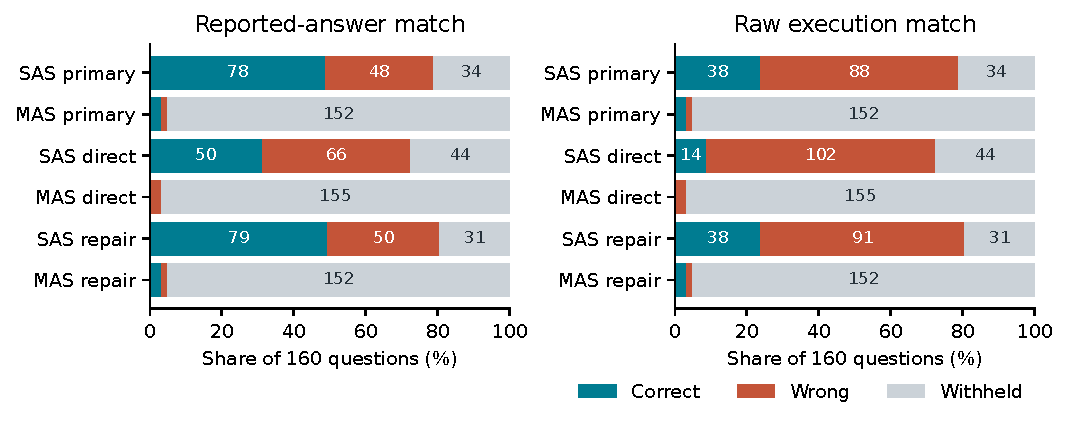
\includegraphics[width=\textwidth]{figures/tier16_outcomes.pdf}
\caption{Study A: all six completed Ubuntu jobs, each on the same 160 questions. Segments show correct (teal), wrong (orange) and withheld (gray); labels are counts where space permits. Both scoring conventions are retained. Fewer MAS errors accompany substantially lower correct delivery.}
\label{fig:tier16}
\end{figure*}
The primary SAS delivers 78 correct, 48 wrong and withholds 34 under reported-answer scoring; MAS delivers 5 correct, 3 wrong and withholds 152 (Figure~\ref{fig:tier16}). The MAS-minus-SAS correct-delivery difference is $-45.6$ percentage points, with a report-cluster 95\% interval $[-53.9,-36.6]$. Raw execution matching changes SAS correct delivery to 38 and wrong delivery to 88, while MAS remains at 5 and 3. Thus the direction is robust to these scores, but the magnitude is not interchangeable across them.

Reported-score transitions are SAS-correct to MAS-correct/wrong/withheld: 5/1/72; SAS-wrong: 0/2/46; SAS-withheld: 0/0/34. Thus 46 avoided wrong deliveries accompany 72 lost correct deliveries through withholding, plus one correct-to-wrong transition. SAS has higher correct delivery on 33 reports, ties on 17, and loses on none. This is specific to reported scoring: raw scoring has one MAS-only correct answer. Conditional precision is 78/126 versus 5/8 (61.9\% versus 62.5\%), at 78.8\% versus 5.0\% coverage; similar precision does not establish equivalent usefulness. The other report-cluster effects are reported wrong $-28.1$ pp [$-37.1,-20.1$], raw correct $-20.6$ [$-28.3,-13.4$], and raw wrong $-53.1$ [$-61.9,-44.1$]. Company clustering and alternative weighting preserve these directions (supplement).

Candidate analysis locates the primary failure. SAS produces 150 executable candidates, 84 reported-correct; review withholds six correct and 18 executable wrong candidates. MAS produces only ten executable candidates, five reported-correct; it delivers all five correct and three wrong, withholding two executable wrong candidates. Its other 150 program-stage outputs are INSUFFICIENT, although all 160 responses parse as JSON. The team is therefore mainly generation-limited, not a strong solver hidden behind an excessively conservative final gate.

All annotated evidence spans occur in 138/160 packets. Within that reference-dependent stratum, SAS delivers 74 correct answers and MAS five; MAS still has 128 insufficient/invalid outputs. This descriptive audit does not prove unique catalog expressibility or causal sufficiency of retrieval. It does show that missing annotated spans alone cannot explain the observed coverage collapse.

For example, AAPL/2003/page\_24.pdf-1 supplies 290 and 92 in the selected sentence. SAS subtracts them to obtain the reference 198; MAS selects the sentence but emits INSUFFICIENT. Conversely, on PNC/2018/page\_171.pdf-1 the team passes a source-cited but numerically wrong calculation. These traces illustrate separate generation and verification failures; they do not isolate model capacity as their cause. The grammar lacks direct aggregate operations, and MAS withholds all 56 cases whose reference programs have multiple steps. Full traces and reference-defined strata appear in the supplement.

Direct control yields SAS 50/66/44 and MAS 0/5/155 correct/wrong/withheld. Repair yields SAS 79/50/31 and MAS 5/3/152. Initial candidates match the no-repair primary across paired cases. SAS repair releases one additional reported-correct and two wrong answers; by raw execution it releases zero correct and three wrong. MAS attempts 152 repairs without improving final delivery. More stages do not resolve the observed generation shortfall.

The Ubuntu run repeats all 960 historical delivery flags and score objects. Its 668,817 memory samples across 16 attempts show zero process-swap bytes and a maximum RSS of 10.946 GB, below the 11.5 GB sampled ceiling. This is stronger resource evidence than the earlier swap-affected run, but not uninterrupted execution or a bound on unsampled peaks. Primary SAS/MAS sampled peaks are 10.075/10.946 GB. Summed primary inference time is 11.668 hours for SAS and 3.383 for MAS; the latter's speed accompanies pervasive insufficient answers. Restart overhead and aborted work are excluded.

\subsection{Evidence and Precision Do Not Resolve Generation}
On 96 additional FinQA reports, an annotated correct program can execute from the original evidence/catalog on 82. Each matched 3B Q4 and Q8 condition misses 80 of those 82 and achieves only 2/96 official execution matches overall. The Q4/Q8 comparison has two gains and two losses, with a company-cluster difference interval about $[-4.3,+4.0]$ points. Increasing weight precision does not establish a general gain here; it is not evidence that precision never matters.

Wider lexical retrieval improves complete annotated-span coverage from 750/883 to 827/883 in a development screen. A 16-report generation pilot improves from 1 to 4 official matches, but a separate 21-report replication changes 2 to 1 (one gain, two losses). All three initial gains use only original spans. Expanding the catalog improves an enriched five-report diagnostic from 0 to 2, but changes 2/96 to 1/96 on the broader cohort. Retrieval coverage, catalog expressibility and generated accuracy are distinct outcomes.

The 15-report answer-key diagnostic shows where conditional potential remains (Table~\ref{tab:oracle}). Operand restriction alone leaves accuracy at zero despite reducing the median selectable IDs from 23 to two. Structure alone recovers four answers; structure plus the shortlist recovers ten official matches but seven reported matches. The remaining five official failures assign at least one source slot a different numerical value from the reference; three additional official-correct outputs mislabel a fractional result as percentage points. Because the scaffold supplies most of the calculation, this is not a learned planning result or an upper bound over all valid reasoning strategies.

\begin{table}[t]
\centering
\begin{tabular}{lrr}
\toprule
Constraint ($n=15$) & Execution & Reported\\
\midrule
Neither & 0 & 0\\
Operand shortlist only & 0 & 0\\
Operation structure only & 4 & 4\\
Structure and shortlist & 10 & 7\\
\bottomrule
\end{tabular}
\caption{Enriched FinQA diagnostic, correct candidates. The last three rows use reference information unavailable at deployment. No deployment accuracy claim follows from these scores.}
\label{tab:oracle}
\end{table}

\subsection{The Evidence-Only Planner Fails Its Criterion}
\begin{figure*}[t]
\centering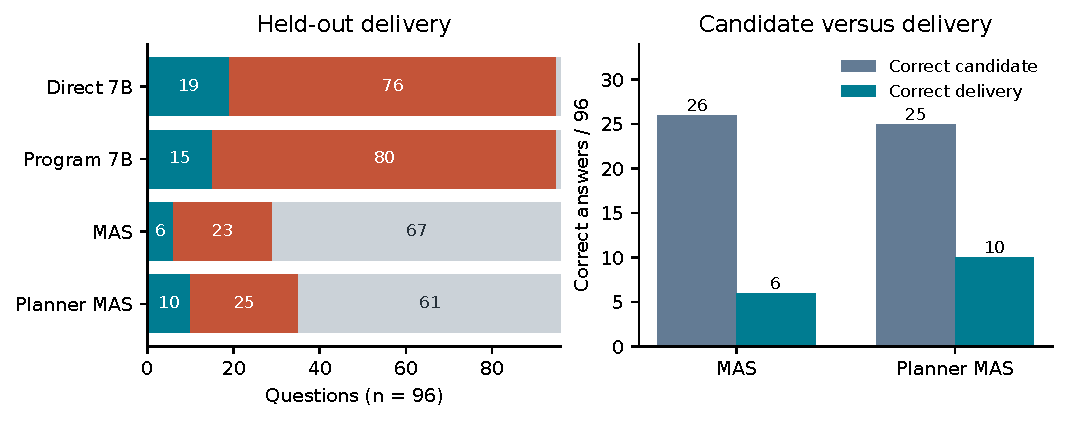
\includegraphics[width=\textwidth]{figures/planner_outcomes.pdf}
\caption{Primary held-out TAT-QA cohort. Left: all correct, wrong and withheld deliveries. Right: correct candidates before review versus correct final deliveries. Planning delivers more correct answers but generates fewer correct candidates and more wrong deliveries.}
\label{fig:planner}
\end{figure*}
All four arms complete the 96-context cohort (Figure~\ref{fig:planner}). Direct 7B delivers 19 correct, 76 wrong and withholds one; program 7B delivers 15, 80 and one. Current MAS delivers 6, 23 and 67; planner MAS delivers 10, 25 and 61. Planning gains four correct deliveries and loses none: $+4.2$ percentage points, paired context-bootstrap 95\% interval $[+1.0,+8.3]$. However, only four pairs are discordant, giving exact $p=0.125$. We do not treat the positive percentile interval as reliable evidence of a population gain. Wrong deliveries increase by two, so the prespecified practical criterion fails regardless of that interval.

Correct candidates decline from 26 to 25, with four gains and five losses. All four candidate gains are delivered. Two gains acquire a matching operator tree; the other two already had matching tree structure and improve numerical binding. Among 87 parseable reference derivations, operator-tree matches fall from 46 to 40 (three gains, nine losses). This diagnostic replaces numerical leaves with placeholders and sorts commutative arguments; it does not recognize all algebraic equivalences or verify source identities. Figure~\ref{fig:effects} reports uncertainty for these paired changes.

\begin{figure}[t]
\centering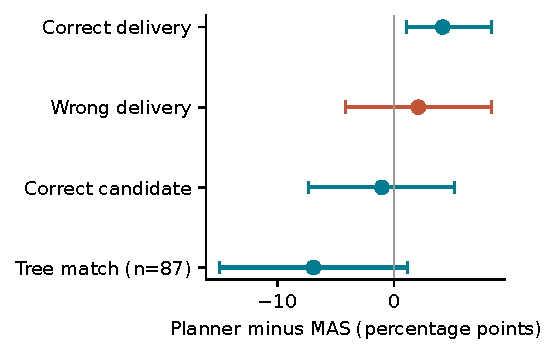
\includegraphics[width=\columnwidth]{figures/planner_effects.pdf}
\caption{Planner-minus-MAS effects with archived 95\% paired context-bootstrap intervals. Correct delivery has only four discordant pairs (exact $p=0.125$). Wrong delivery is an adverse outcome; its observed increase fails the practical criterion. Tree agreement uses 87 parseable cases.}
\label{fig:effects}
\end{figure}
Connected shapes are usable on 57/96 contexts. The other 39 have operations outside the final dependency graph and fall back; all 39 saved drafts and verdicts reproduce the baseline. Passing structural validation does not guarantee a correct calculation. The fixed critic rejects 20 of 26 correct baseline candidates and 15 of 25 planner candidates. Its changed acceptance pattern improves correct delivery without a net generation gain and still accepts 25 wrong planned answers.

On the separate 28-context official-test cohort, both MAS arms deliver two correct, ten wrong and withhold 16; correct candidates decrease from five to three. This is a small negative directional check, not proof of equality. The 7B comparison stops after two contexts because of a 352,342,016-byte CPU compute-buffer allocation failure; a recovery attempt also fails. We retain the partial records but do not report a complete four-arm official-test comparison.

Planning also costs time: median resident request latency increases from 25.2 to 33.9 seconds; generated tokens increase from 6,672 to 9,863. Peak worker commit remains about 5.26 GB (Figure~\ref{fig:resources}). Direct and program 7B medians are 34.3 and 46.8 seconds with approximately 5.44 GB peak commit, but include model loading and are not matched resident latency comparisons.

\begin{figure*}[t]
\centering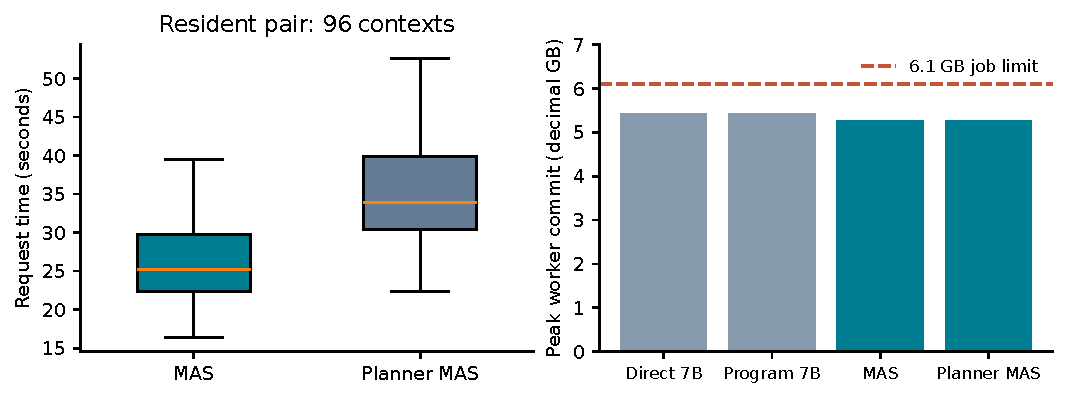
\includegraphics[width=\textwidth]{figures/resources.pdf}
\caption{Primary held-out resources. Left: resident request-time distributions (median, quartiles and 1.5-IQR whiskers; outliers omitted from display, retained in data). Right: observed peak worker commit and configured limit. Peaks are descriptive measurements, not physical-RAM feasibility bounds; cross-arm loading policies differ.}
\label{fig:resources}
\end{figure*}

\subsection{Stronger Baselines and Nontransferable Gains}
The result is not that larger or direct models always fail to help. On 120 fresh TAT-QA contexts, direct 7B scores 29 versus 12 for direct 3B (22 gains, five losses; exact paired $p=0.00151$). An earlier 40-context comparison is inconclusive at six versus five. On the shared 96-report FinQA cohort, fixed 7B direct output scores 35 versus 20 for cited programs under reported-answer matching (21 direct-only, six program-only; $p=0.00592$). In contrast, a 72-context TAT-QA subset favors programs 19 versus 14 (14 program-only, nine direct-only; $p=0.405$). Output-format effects depend on task, representation and scoring; no universal direct-answer advantage is supported.

Scoring sensitivity is substantial. FinQA's unmodified official execution score for those 7B programs is 1/96. A post-hoc declared-percent conversion recovers 18, yielding 19/96; the original score is retained. Three unsupported reported-reference labels remain in denominators. These observations do not license replacing the primary scorer with a favorable convention.

FinQA actor adaptation transfers to 72 other TAT-QA contexts with correct candidates increasing from three to eight (six gains, one loss; $p=0.125$); the critic delivers six correct, ten wrong and withholds 56. On fixed FinQA candidates, an initially favorable trained-critic pilot does not reproduce zero wrong deliveries in a 21-report transfer: control delivers 1/5/15 and crossed critic 1/2/18. Earlier crossed-critic development also fails its no-correct-loss adoption rule against the stronger original critic. These observations remain part of the negative sequence.

The clearest engineering improvement is cache configuration. On a fixed resident 21-report workload, disabling RAM prompt caching preserves every draft, verdict and delivery while reducing peak worker commit from approximately 6.101 to 5.264 GB and eliminating logged prompt-cache allocation failures. The default-cache completion involved allocation fallback near the cap. This change improves observed resource headroom, not reasoning accuracy, and does not prove absence of Windows paging.

\section{Discussion and Limitations}
The evidence supports a sequence of distinct constraints. In Study A, the selected F16 team generally does not attempt a useful calculation. In Study B, available reference-executable evidence can coexist with wrong candidate programs. Supplying reference structure exposes conditional potential, but predicting usable structure remains difficult, source assignment can still fail, and review can discard correct candidates or accept wrong ones. The planner's final delivery increase is therefore insufficient evidence of a generation improvement.

This is an empirical result about specific Qwen2.5 recipes, prompts, grammars and financial subsets. Parameter size and precision are confounded in Study A; the Windows planner changes draft allocation as well as adding a stage. Greedy single-seed experiments do not estimate training-seed or stochastic-decoding variance. Repeated development studies, enriched oracle diagnostics and reused cohorts cannot be pooled as independent confirmations. Project-held-out public data do not establish freedom from pretraining contamination; FinQA splits overlap at report level, and TAT-QA report clusters are unavailable. Sparse paired improvements and multiple exploratory comparisons limit inferential strength.

Resource claims are equally bounded. Windows job commit is not physical RAM feasibility; sampled RSS can miss peaks. Linux swap-disabled scope records and zero sampled process swap strengthen the Ubuntu evidence, but the run was interrupted and the SSD suffered filesystem errors. Seven unreadable analysis artifacts were reconstructed offline: all six replay hashes and all 40 recorded evidence hashes match, as does the regenerated summary; the regenerated text report has no original recorded hash. The original export tarball and one bootstrap log remain unavailable. Separately verified repository archives preserve the usable evidence. These qualifications preclude claims of uninterrupted deployment reliability.

We have not evaluated frontier models, alternative families, a broad prompt search, trained planners, XBRL-authorized formulas, or all published verification baselines. We report numerical benchmark agreement rather than expert financial adjudication, calibration or operational safety. Full prompts may contain ambiguity, and correct numbers do not ensure correct provenance. The systems' error rates do not support autonomous financial decisions. The supplement retains historical positive, null and adverse findings, unsuccessful resource attempts and a machine-readable artifact census; no historical result is silently revised.


\section{Conclusion}
The observed errors cannot be summarized by one accuracy number. The F16 team loses useful coverage; reference-informed constraints reveal conditional recovery; evidence-only planning fails its practical requirement. Research on local financial reasoning should therefore measure candidate quality and delivery together, preserve scorer sensitivity, and treat resource feasibility as a separate empirical claim.

\section*{Supplementary Materials}
The accompanying comprehensive technical supplement retains the complete historical condition census, paired uncertainty and sensitivity analyses, candidate/delivery transitions, conditional mathematical results, worked failure examples, and reproduction details. It is the preserved, audited supporting manuscript; no experimental outcome is changed in this journal adaptation.

\section*{Required author declarations}
Author contributions, funding, conflicts of interest and approval statements require completion by the actual authors. No facts about them are inferred. Data/code availability must identify the accessible evidence archives and disclose the missing original export/log artifacts. This draft is not ready for submission until those declarations are reviewed.
\section*{Automated assistance and author responsibility}
This draft was prepared with AI-assisted manuscript adaptation, code-based numerical checking and plotting using the preserved research record. Human authors must review the scientific text, establish authorship and complete applicable disclosures before submission. No new research-model inference was performed during manuscript preparation.

\bibliography{references}
\end{document}
